%----------------------------------------------------------------------------------------
%	RESULTS
%----------------------------------------------------------------------------------------
% TODO divide into subsections: Results for Agent, Results for Experiment, Comparison
% TODO make a 3x2 grid with different risks.

\large{Solving the risk sensitive POMDP}

\normalsize

State space must be augmented two times:
\begin{figure}
\begin {center}
\begin {tikzpicture}[-latex ,auto ,node distance =3cm and 4cm ,on grid ,
semithick ,
state/.style ={ circle ,fill=black!20, minimum width =3 cm}]
\node[state] (A) [align=center] {Reces\\sion};
\node[state] (B) [right of=A,align=center] {Boom\\ing};
\node[state] (C) [right of=A,align=center] {$Sold$};

\coordinate[below of=A] (AA);
\coordinate[below of=B] (BB);
\coordinate[below of=AA] (D);
\coordinate[below of=BB] (E);


\path (A) edge [loop left, line width=2mm, align=center] node[left] {wait \\ $0.86$} (A);
\path (A) edge [bend left = -25,line width=2mm,align=center] node[below =0.25 cm] {sell\\$1.0$} (C);
\path (A) edge [bend left =25,line width=2mm,align=center] node[above] {wait\\$0.14$} (B);

\path (B) edge [loop right,line width=2mm,align=center] node[right] {wait\\$1.0$} (B);
\path (B) edge [bend right = -25,line width=2mm,align=center] node[below =0.25 cm] {sell\\$1.0$} (C);

%\fill[gray!40!white, opacity=0.5] (-6,-1) rectangle (5,6);

\path (A) edge [bend right =25,line width=2mm, dashed] node[left] {$Observation$} (D);
\path (B) edge [bend left  =25,line width=2mm, dashed] node[right] {$Observation$} (E);
\end{tikzpicture}
\end{center}
\end{figure}


Observation and time to belief and time
belief and time to belief and wealth

\cite{marecki} showed that in belief time space POMDPs can be solved for arbitrary utility functions using \textbf{reverse value iteration}.

\begin{figure}
    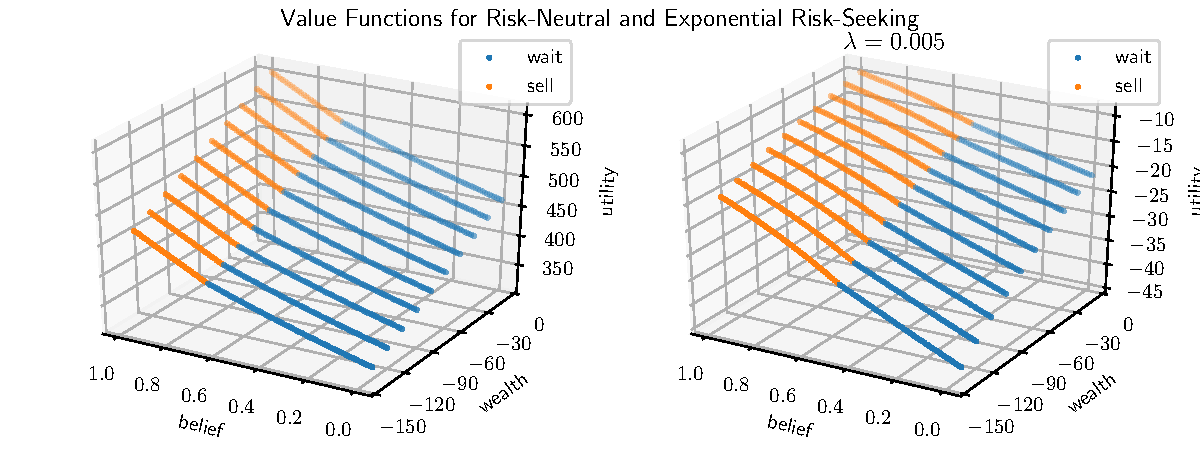
\includegraphics[width=0.9\linewidth]{img/exp_policy.pdf}\\
    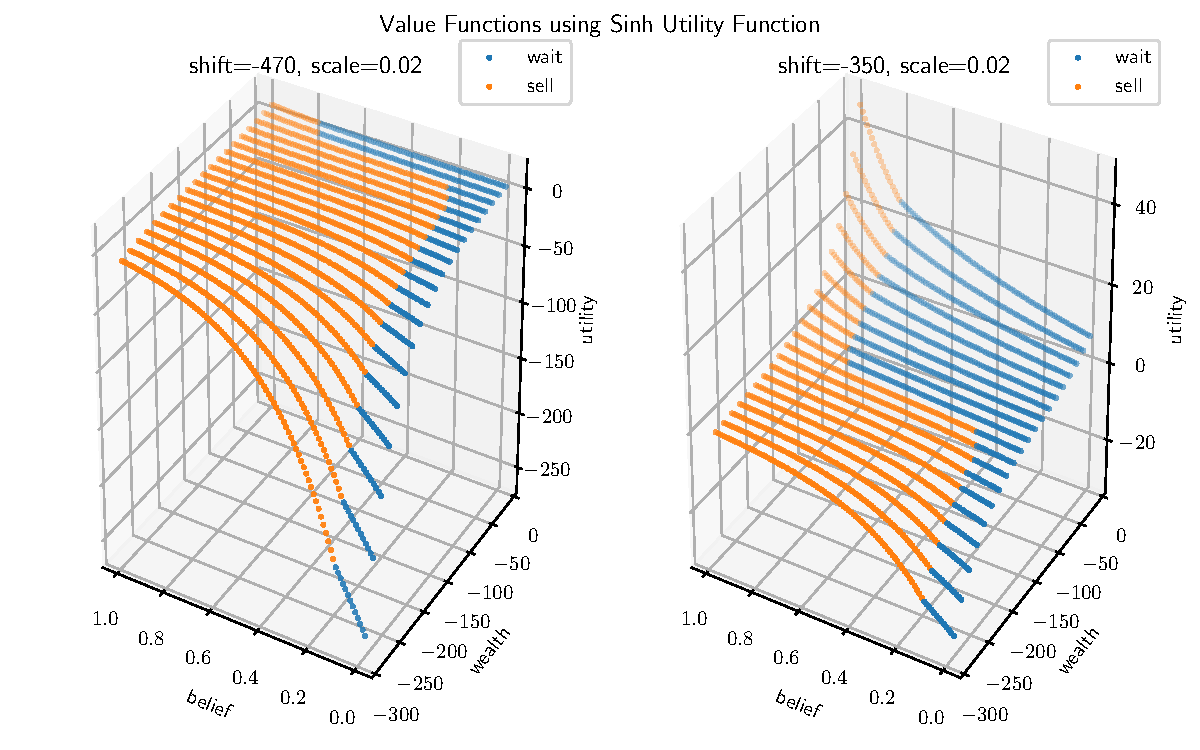
\includegraphics[width=0.9\linewidth]{img/sinh_policy.pdf}\\
    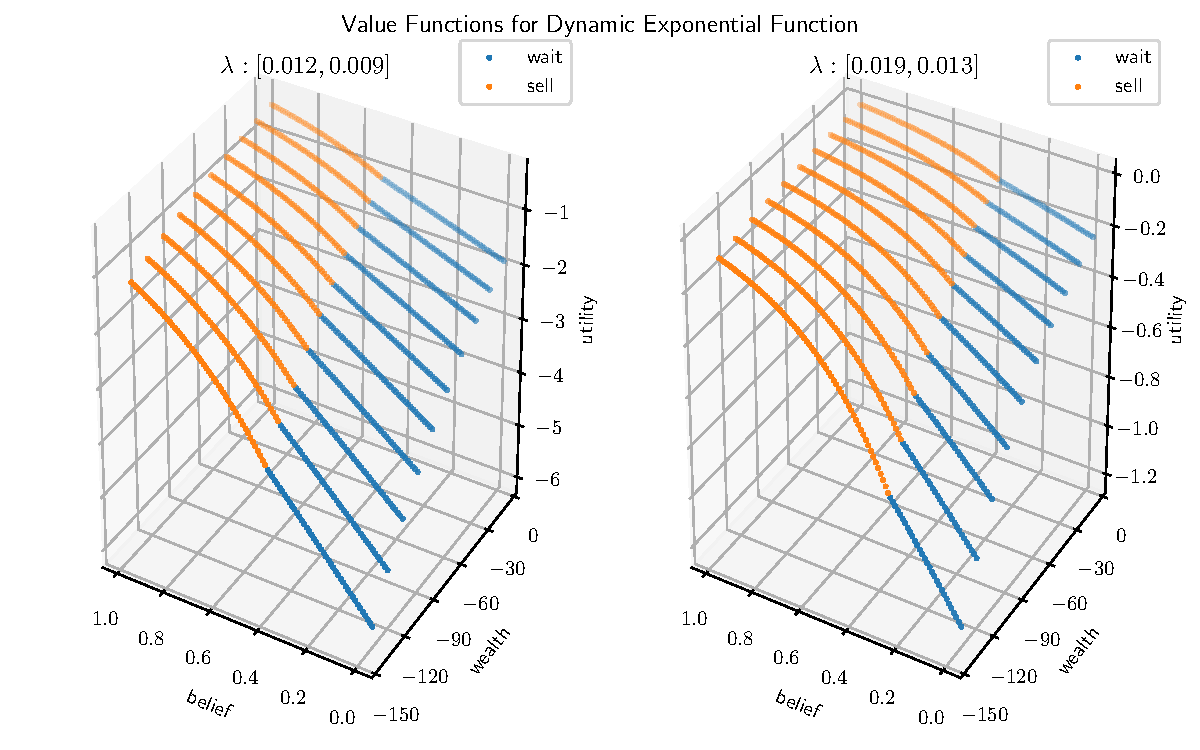
\includegraphics[width=0.9\linewidth]{img/dyn_policy.pdf}
    \caption{Value functions exhibiting different risk-behaviors; from top left: risk neutral agent (utility function is the identity function), risk-seeking agent with exponential utility function, two fixed time agents with different time thresholds, two agents with dynamic exponential utility function in the expensive expert scenario.}
\end{figure}

\textbf{The original problem:}
\begin{itemize}
\item[①] Choose utility function with risk parameter.
\item[②] Perform value iteration.
\item[③] Derive policy.
\end{itemize}

\textbf{The inverse problem:}
\begin{itemize}
\item[①] Observe behavior.
\item[②] Estimate policy.
\item[③] Derive utility function and risk parameters.
\end{itemize}

The original problem is easy to solve, unfortunately for the inverse problem no solution is known. $\rightarrow$ Perform grid-search and choose optimal utility function.
